\documentclass{jsce-word}

\title{INSTRUCTION TO THE AUTHORS OF JOURNAL OF SCIENCE AND ENGINEERING\\
  {[TYPE THE TITLE OF YOUR PAPER HERE]}}
\author{Name of Author\textsuperscript{1}, Name of Author\textsuperscript{2}}
\affiliation{\textsuperscript{1}Affiliation\\\textsuperscript{2}Affiliation}
\corresponding{Name of an author\\
  Affiliation of the corresponding author\\
  Email: email of the corresponding author}
\keywords{Up to 5 words must be carefully selected to facilitate reader's search separated by commas.}
\runningauthor{Author}

\begin{document}

\begin{abstract}
This draft illustrates preparation of your paper using MS-WORD. All papers should be
submitted as MS-WORD documents not exceeding to 8 pages. The abstract should not exceed 200
words and must precise the paper giving clear conclusions in 10.5 point. It should briefly
summarize the essence of the paper and address the following areas without using
subsections: Objective - briefly state the problem or issue addressed in language accessible
to a general scientific audience. Method - briefly summarize the technological innovation or
method used to address the problem. Results - provide a short statement of the results and
findings. Conclusions - give brief concluding remarks on your outcomes. Detailed discussion
of all these aspects should be provided in the main body of the paper. Authors are
encouraged to refer the JScE manuscript template for manuscript preparation which is
available at JScE homepage---INSTRUCTION TO AUTHORS.
\end{abstract}

\maketitle

\section{Manuscript Format Guidelines}

The main body of the text will have a good introduction of the paper at the beginning.
Simple language, short sentences and good use of section headings help to communicate
information more effectively. Figures are important in aiding the clarity of the paper.

\subsection{Type Area}
The manuscript should be printed in A4 size paper with 25 mm margin on top and bottom and
20 mm on right and left.

\subsection{Script}
The manuscript must use Times Roman of 10.5 font size in English and 10.5 fonts in Nepali.

Adjust line spacing to accommodate 50 lines in the page. Hand written manuscripts will not
be accepted. Number all pages starting with the title page. Please leave one blank space
(10.5 pt.) between each of the following: title, author's names, address, and abstract.

All subsequent paragraphs should be indented as here with no line spacing between
paragraphs. Two line spaces (10.5 pt.) should follow each section.

\subsection{Title Page}
The first page must contain the title of the paper, author full name (s), affiliation (s),
position (s) and contact author's name, position, affiliation and mailing address, phone and
fax numbers and email address.

\subsection{Length}
Papers should not exceed 8 pages length including figures, tables, endnotes and references.

\subsection{Equations}
Equations should be written in Equation Editor/Math Type, numbered consecutively beginning
with (1) throughout the paper. The number should be enclosed in parenthesis and set flush
right in the column on the same line of the equation. Example is shown below.
\begin{equation}
  \sum_{e\in\delta^{+}(i)}\int_{0}^{T} f(e,\theta)\,d\theta
  = \sum_{e\in\delta^{-}(i)}\int_{0}^{T} f(e,\theta)\,d\theta.
\end{equation}

\subsection{Figures}
Insert the figures in the text and arrange them consecutively in Arabic numerals, e.g.,
Fig. 1, Fig. 2 etc. Original figures should be included in the final submission. Make sure
all type face in the figure is legible when reduced to the size for publication. Pictures
should be in JPEG format. Sample has been shown in Fig.~\ref{fig1}.

\begin{figure}[H]
  \vspace*{28.6pt}
  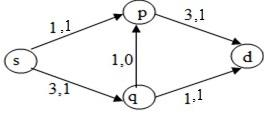
\includegraphics[width=195pt,height=90.7pt]{figures/fig1.jpg}
  \caption{Caption of the figure.}
  \label{fig1}
  \vspace{-11.6pt}
\end{figure}

\subsection{Measurements}
International system of units (SI) should be used. If other units are used, equivalents
should be given in parenthesis.

\begin{table*}[b]
  \caption{Title of Table}
  \label{tab1}
  \centering
  \setlength{\tabcolsep}{5.4pt}
  \begin{tabular}{|m{99.7pt}|m{99.7pt}!{\vrule width 1.5pt}m{99.7pt}|m{99.7pt}|}
    \hline
    \multicolumn{2}{|c!{\vrule width 1.5pt}}{\rule[-4.3pt]{0pt}{14.4pt}Format for Table} & \multicolumn{2}{c|}{} \\
    \hline
    \rule[-4.3pt]{0pt}{23.5pt} & & & \\
    \hline
    \rule[-4.3pt]{0pt}{42.1pt} & & & \\
    \hline
    \rule[-4.3pt]{0pt}{23.6pt} & & & \\
    \hline
  \end{tabular}
  \vspace{4.6pt}
\end{table*}

\subsection{Tables}
Insert tables in the text and number them consecutively in Arabic numerals, e.g., Table 1,
Table 2 etc. as shown in Table~\ref{tab1} below.

\section{Major Sections and Headings}

Though, the organization of the body of the paper is at the authors' discretion, and may
slightly be deviated according to the research areas; the only required sections are
Introduction, Literature, Methods/ Procedures, Results, Conclusion and References.
Acknowledgement (just before the Reference) and Appendices (just after the Reference) are
optional. Each of the headings and subheadings should be numbered in numerals with
bold-faced. The section headings will indicate hierarchy levels such as 2, 2.1, 2.1.1.
Hierarchy of more than three is not preferred.

\section{Citing References}

References in the text should be quoted giving the last name of the author(s) and the year
of publication of the reference in the following manner: \citet{karanjit2017} for single
author, \citet{khadka2017} for two authors and \citet{burkard1993} for more than two authors
or \citep{karanjit2017} for single author, \citep{khadka2017} for two authors and
\citep{burkard1993} for more than two authors respectively. The style should follow the
examples as given in \textbf{Reference} Section. This section also provides example of
referencing the book, proceedings, thesis and links.

\nocite{*}
\bibliographystyle{jsce-word}
\bibliography{references}

\textbf{Endnotes}: A limited number of explanatory notes are permissible. These should be
numbered 1, 2, 3 consecutively in the text and denote by superscripts. Endnotes should be
listed at the end of the paper with numbers linked to those in the text.

\end{document}
